\section{Time stepping methods}\index{time stepping}

% \subsection{Mid-point rule}

\subsection{Adams Predictor-Corrector}\index{time stepping!Adams predictor corrector}

{
\newcommand{\figWidtha}{.475\linewidth}
\begin{figure}[hbt]
  \begin{center}
%   \epsfig{file=\obFigures/adamsPECE22.ps,width=.475\linewidth}
%   \epsfig{file=\obFigures/adamsPECE44.ps,width=.475\linewidth}
   \includegraphics[width=\figWidtha]{./fig/adamsPECE22}
   \includegraphics[width=\figWidtha]{./fig/adamsPECE44}
  \end{center}
\caption{Stability regions for the predictor corrector methods. Left: second-order method, PECE mode.
         Right: fourth-order method, PECE mode.} \label{fig:pcStabilityRegion}
\end{figure}
}

If we write the INS equations as
\[
      \uv_t = \fv(\uv,p)
\]
where we may think of the pressure $p$ as simply a function of $\uv$ and we may use any time integrator
in a method-of-lines fashion.

The {\bf second-order accurate Adams predictor-corrector} time stepping method for the INS equations can be chosen
with the ``{\tt adams PC}'' option. 
It is defined by 
\begin{align*}
 { \uv^p - \uv^n \over \dt } &= {3\over2} \fv^n - \half\fv^{n-1} \\
 { \uv^{n+1} - \uv^n \over \dt } &= {1\over2} \fv^p + \half\fv^n
\end{align*}
where we have shown one correction step (one may optionally correct more than one time).
The stability region for this method is shown in figure~(\ref{fig:pcStabilityRegion}).

To allow for a time-step that may change we actually use
\begin{align*}
 { \uv^p - \uv^n \over \dt } &= p_0 \fv^n + p_1 \fv^{n-1} \\
 { \uv^{n+1} - \uv^n \over \dt } &= {1\over2} \fv^p + \half\fv^n \\
 p_0 &= 1 + \dt/(2 \dt_1) \\
 p_1 &= -\dt/(2 \dt_1)  
\end{align*}
where $\dt_1=t_n-t_n-1$.


The {\bf fourth-order accurate Adams predictor-corrector} time stepping method for the INS equations can be chosen
with the ``{\tt adams PC order 4}'' option. 
It is defined by 
\begin{align*}
 { \uv^p - \uv^n \over \dt } &= {1\over 24}\Big[ 55 \fv^n -59\fv^{n-1} +37\fv_{n-2}-9\fv_{n-3}\Big] \\
 { \uv^{n+1} - \uv^n \over \dt } &= {1\over 24}\Big[ 9\fv^p + 19\fv^n -5\fv^{n-1} +\fv_{n-2}\Big]
\end{align*}
(see for example Lambert\cite{Lambert73}).
The stability region for this method is shown in figure~(\ref{fig:pcStabilityRegion}).

To allow for a time-step that may change we actually use
\begin{align*}
 { \uv^p - \uv^n \over \dt } &=  p_0 \fv^n +p_1 \fv^{n-1} + p_2\fv_{n-2} +p_3 \fv_{n-3} \\
 { \uv^{n+1} - \uv^n \over \dt } &= c_0 \fv^p + c_1\fv^n +c_2\fv^{n-1} + c_3\fv_{n-2}  \\
 p_0 =& (6 \dt_0 \dt_2 \dt_2+12 \dt_2 \dt_2 \dt_1+8 \dt_0 \dt_0 \dt_2+24 \dt_2 \dt_0 \dt_1+ \\
      &   12 \dt_2 \dt_1 \dt_3+6 \dt_3 \dt_2 \dt_0+24 \dt_1 \dt_1 \dt_2+12 \dt_0 \dt_3 \dt_1+18 \dt_0 \dt_1 \\
      &	\dt_1+4 \dt_0 \dt_0 \dt_3+12 \dt_1 \dt_1 \dt_3+3 \dt_0 \dt_0 \dt_0+12 \dt_0 \dt_0 \dt_1+12 \dt_1\\
	      &        \dt_1 \dt_1) \dt_0/(\dt_1+\dt_2+\dt_3)/\dt_1/(\dt_1+\dt_2)/12  \\
 p_1 =& -\dt_0 \dt_0 (6 \dt_1 \dt_1+6 \dt_3 \dt_1+12 \dt_2 \dt_1+8 \dt_0 \dt_1+3 \dt_0 \\
      &	\dt_0+6 \dt_2 \dt_3+4 \dt_0 \dt_3+8 \dt_2 \dt_0+6 \dt_2 \dt_2)/\dt_1/(\dt_2+\dt_3)/\dt_2/12  \\
 p_2 =& \dt_0 \dt_0 (6 \dt_1 \dt_1+6 \dt_2 \dt_1+6 \dt_3 \dt_1+8 \dt_0 \dt_1+3 \dt_0 \dt_0 \\
      &		       +4 \dt_2 \dt_0+4 \dt_0 \dt_3)/\dt_3/\dt_2/(\dt_1+\dt_2)/12  \\
 p_3 =& -(6 \dt_1 \dt_1+6 \dt_2 \dt_1+8 \dt_0 \dt_1+4 \dt_2 \dt_0+3 \dt_0 \dt_0) \dt_0 \\
      &                        \dt_0/(\dt_1+\dt_2+\dt_3)/(\dt_2+\dt_3)/\dt_3/12  \\
 c_0 =& (6 \dt_1 \dt_1+6 \dt_2 \dt_1+8 \dt_0 \dt_1+4 \dt_2 \dt_0+3 \dt_0 \dt_0) \\
      &  \dt_0/(\dt_0+\dt_1+\dt_2)/(\dt_0+\dt_1)/12  \\
 c_1 =&  \dt_0 (\dt_0 \dt_0+4 \dt_0 \dt_1+2 \dt_2 \dt_0+6 \dt_1 \dt_1+6 \dt_2 \dt_1)/(\dt_1+\dt_2)/\dt_1/12  \\
 c_2 =&  -\dt_0 \dt_0 \dt_0 (\dt_0+2 \dt_1+2 \dt_2)/(\dt_0+\dt_1)/\dt_2/\dt_1/12  \\
 c_3 =&  (\dt_0+2 \dt_1) \dt_0 \dt_0 \dt_0/(\dt_0+\dt_1+\dt_2)/(\dt_1+\dt_2)/\dt_2/12 
\end{align*}
where $\dt_m=t_{n+1-m}-t_{n-m}$, $m=0,1,2,3$.

\subsection{Implicit multistep method with viscous terms implicit} \label{sec:implicitMultiStep}\index{time stepping!implicit multistep}

  With the {\tt implicit} time stepping method the INS equations are integrated with
the viscous terms treated implicitly and the other terms treated with a 2nd-order
Adams predictor corrector.
If we split the equations into an explicit and implicit part,
\begin{align*}
  \uv_t &= \left[ -(\uv\cdot\grad)\uv -\grad p \right] + \nu\Delta \uv \\
  \uv_t &= \fv_E + A \uv  \\
   \fv_E &= -(\uv\cdot\grad)\uv -\grad p \\
   A \uv &= \nu\Delta \uv
\end{align*}
then the time step consists of a predictor,
\[
 { \uv^p - \uv^n \over \dt }= {3\over2} \fv_E^n - \half\fv_E^{n-1} + \alpha A \uv^p + (1-\alpha)A\uv^n  
\]
and a corrector
\[
 { \uv^c - \uv^n \over \dt }= {1\over2} \fv_E^p + \half\fv_E^{n} + \alpha A \uv^c + (1-\alpha)A\uv^n 
\]
The {\tt implicit factor} $\alpha$ can be set as a parameter. A value of $\alpha=\half$ will give a
second-order Crank-Nicolson method. A value of $\alpha=1$ will give a first-order backward-Euler method.




% -----------------------------------------------------------------------------------------------------------
\subsection{Implicit multistep method with the viscous and non-linear terms implicit} 
\label{sec:implicitMultiStepNonlinear}\index{time stepping!implicit multistep}

\newcommand{\uvl}{\uv^*} % linearized state

Consider now the case of treating the viscous and non-linear terms in an implicit manner.

In the general case we are solving a nonlinear equation of the form
\begin{align*}
  \uv_t & = \fv(\uv) .
\end{align*}  
We linearize a part of the operator $\fv(\uv)$ around the state $\uvl(\xv,t)$ and write the equation as
\begin{align}
  \uv_t & = L(\uv; \uvl) + \big( \fv(\uv) - L(\uv; \uvl) \big) \\  \label{eq:equationWithLinearLinearizedTerm}
        & = L(\uv; \uvl) + \fv_E(\uv; \uvl) 
\end{align} 
where
\begin{align}
  \fv_E(\uv; \uvl) & \equiv \fv(\uv) - L(\uv; \uvl)
\end{align}  
Here $L(\uv; \uvl)$ is a linear operator of $\uv$ that depends upon $\uvl$.
For example if $\fv(\uv)=(\uv\cdot\grad)\uv$ then one choice could be
$ L(\uv; \uvl) = (\uvl\cdot\grad)\uv$.  Another choice could be 
$ L(\uv; \uvl) = (\uvl\cdot\grad)\uv + (\uv\cdot\grad)\uvl$.
% 
We can now define a implicit time-stepping method that uses the form~\eqref{eq:equationWithLinearLinearizedTerm}.
% 
A backward-Euler approximation to the full equations is
\begin{align*}
{ \uv^{n+1} - \uv^n \over \dt } &= L(\uv^{n+1}; \uvl) + \fv_E(\uv^{n+1}; \uvl)  ~.
\end{align*} 
This equation can be solved by {\em implicit} iteration (treating the $L$ term implicitly),
\begin{align*}
{ \vv^k - \uv^n \over \dt } &= L(\vv^k; \uvl) + \fv_E(\vv^{k-1}; \uvl) 
\end{align*}  
where we take $\vv^0=\uv^n$ and iterate on $k=0,1,2,...$ for some number of steps. If we iterate until convergence then
we will have solved the original equations with backward-Euler, independent of the choice $L$ and $\uvl$,
\begin{align*}
{ \uv^{n+1} - \uv^n \over \dt } &= \fv(\uv^{n+1})  ~.
\end{align*} 
Of course for best convergence for a large value of $\dt$, we want make good choices for $L$ and $\uvl$.






We could also solve the equations with the trapezodial like rule 
\begin{align*}
{ \uv^{n+1} - \uv^n \over \dt } &= \alpha \fv(\uv^{n+1}) + (1-\alpha) \fv(\uv^n) \\
          &= \alpha L(\uv^{n+1}; \uvl) + (1-\alpha)L(\uv^{n}; \uvl)
                                   +\alpha \fv_E(\uv^{n+1}; \uvl) + (1-\alpha) \fv_E(\uv^n; \uvl), \\
          &= \alpha L(\uv^{n+1}; \uvl) +\alpha \fv_E(\uv^{n+1}; \uvl) + (1-\alpha) \fv(\uv^n) \\
          &= \alpha L(\uv^{n+1}; \uvl) +\alpha\big( \fv(\uv^{n+1}) -L(\uv^{n+1}; \uvl) \big) + (1-\alpha) \fv(\uv^n) 
\end{align*} 
where $\alpha=\half$ is the trapezodial rule and $\alpha=1$ is backward-Euler.
This equation can be solved by the implicit iteration 
\begin{align*}
{ \vv^k - \uv^n \over \dt } &=  \alpha L(\vv^{k}; \uvl) +\alpha\big( \fv(\vv^{k-1}) -L(\vv^{k-1}; \uvl) \big) + (1-\alpha) \fv(\uv^n) 
\end{align*}  
% 
For $\alpha=1/2$, the first iterate $\vv^1$ is second-order accurate in the implicit part $L$ and first order accurate in the
explicit part $\fv_E$. If $\fv_E(\uv^n;\uvl)={\mathcal O}(\dt)$ then the $\vv^1$ is second-order accurate. 
For $\alpha=1/2$ the second and later iterates, $\vv^k$, $k\ge 2$, should be second-order accurate. 


To implement this scheme we need to (1) build the matrix $M$ for the implicit operator,
\begin{align*}
  M \vv^k = (I - \alpha\dt A(\uvl) )\vv^k = \vv^{k}-\alpha\dt L(\vv^{k}; \uvl)
\end{align*} 
(2) evaluate the right-hand-side $\fv(\vv)$, and (3) evaluate the linearized operator $L(\vv; \uvl)$ or
the combination $\fv(\vv) -L(\vv; \uvl)$. 




We could use a predictor step with an second-order accurate explicit predictor for $\fv_E$, 
\begin{align*}
{ \uv^{p} - \uv^n \over \dt }
          &= \alpha L(\uv^{n+1}; \uvl) + (1-\alpha)L(\uv^{n}; \uvl)
                                   + \frac{3}{2} \fv_E(\uv^{n}; \uvl) - \half \fv_E(\uv^{n-1}; \uvl) .
\end{align*}
With $\alpha=1/2$ the predicted value $\uv^{p}$ would be second order. 



\subsection{Example linearizations}


Here is an example for the INS:
\begin{align*}
  \fv(\uv) & = \nu\Delta \uv - (\uv\cdot\grad)\uv - \grad p \\
  L(\uv; \uvl) &= \nu\Delta \uv - \Big( (\uvl\cdot\grad)\uv + (\uv\cdot\grad)\uvl  \Big) \\
 \fv_E(\uv;\uvl) &= \fv(\uv) - L(\uv; \uvl) \\
                 & = - (\uv\cdot\grad)\uv - \grad p + \Big( (\uvl\cdot\grad)\uv + (\uv\cdot\grad)\uvl  \Big)\\
    &= - \grad p  - ((\uv-\uvl)\cdot\grad)(\uv-\uvl) + (\uvl\cdot\grad)\uvl
\end{align*}  

When the viscosity is a function of $\uv$, $\nu=\nu(\uv)$, we could use
Here is an example for the INS:
\begin{align*}
  \fv(\uv) & = \grad\cdot(\nu(\uv)\grad\uv) - (\uv\cdot\grad)\uv - \grad p \\
  L(\uv; \uvl) &= \grad\cdot(\nu(\uvl)\grad\uv)  + \grad\cdot(\nu(\uv)\grad\uvl)
         - \Big( (\uvl\cdot\grad)\uv + (\uv\cdot\grad)\uvl  \Big) \\
 \fv_E(\uv;\uvl) &= \fv(\uv) - L(\uv; \uvl)  \\
                 &= \grad\cdot(\nu(\uv)\grad\uv) - \grad\cdot(\nu(\uvl)\grad\uv)  - \grad\cdot(\nu(\uv)\grad\uvl) \\
              & ~~- (\uv\cdot\grad)\uv - \grad p + \Big( (\uvl\cdot\grad)\uv + (\uv\cdot\grad)\uvl  \Big)\\
    &= \grad\cdot((\nu(\uv)-\nu(\uvl))\grad(\uv-\uvl)) - \grad\cdot(\nu(\uvl)\grad\uvl) \\
        & ~~ - \grad p  - ((\uv-\uvl)\cdot\grad)(\uv-\uvl) + (\uvl\cdot\grad)\uvl
\end{align*} 



% ----------------------------------------------------------------------------------------------------------------
\subsection{Variable time stepping}\index{variable time stepping}

 The {\tt variableTimeStepAdamsPredictorCorrector} time stepping option allows each grid to have
it's own time step. 

